\chapter{Experimentos e Resultados}
\label{chap:resultados}
% ----------------------------------------------------------
Este capítulo vem apresentar os experimentos realizados como forma de
verificação do Processo de Avaliação de Capacidade por Inferência de 
Desempenho proposto no Capítulo~\ref{chap:processo}. Inicialmente é
apresentada a metodologia utilizada para construção dos experimentos, 
com a descrição da Aplicação sob Teste escolhida, como foi implantada e 
como foram realizadas as execuções para coleta de dados de desempenho. Depois
são apresentados os resultados obtidos por cada uma das 9 Heurísticas ao
fazer a Avaliação de Capacidade da Aplicação. Esses resultados são usados 
para uma comparação qualitativa das Heusrísticas entre si e para atestar
a eficiência do Processo de Avaliação de Capacidade proposto e sua técnica 
de Inferência de Desempenho tanto quanto à economia de tempo e custo como  
quanto à precisão de acerto de seuas predições.

\section{Metodologia}
\label{sec:resultados_metodologia}
A fim de validar a eficiência da Inferência de Desempenho no apoio
ao Planejamento de Capacidade, foram realizadas seções de avaliação de
capacidade de uma aplicação implantada em um provedor de nuvem de
infraestrutura como serviço.

A aplicação escolhida foi o WordPress \cite{wordpress}, um motor de construção 
e administração de \emph{blogs}. Sua escolha foi motivada por ser uma aplicação
bem conhecida, de utilização via web, ideal para implantação em ambiente de
nuvem, e com componentes arquiteturais escaláveis. Além disso, o fluxo de 
utilização típico apresenta características bem diversificadas quanto ao uso
de recursos de CPU e memória, rede, sistema de arquivos e banco de dados.

\begin{figure}[hbt]
  \caption{\label{fig:implantacao}Implantação do WordPress na AWS EC2 para Avaliação de Capacidade}
  \begin{center}
    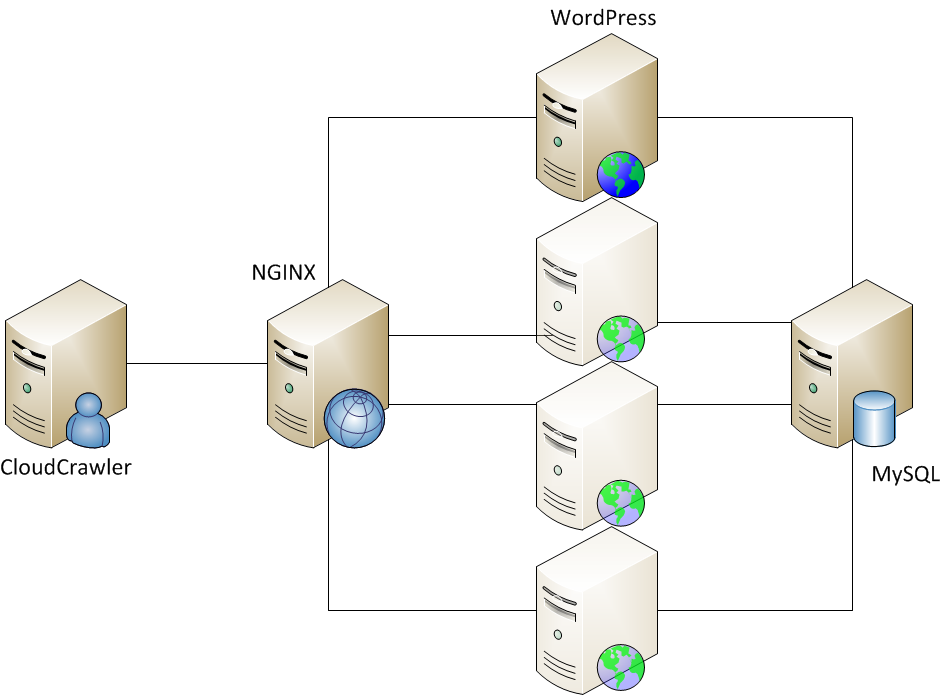
\includegraphics[scale=0.4]{img/ImplantacaoWordPress}
  \end{center}
\end{figure}

O Provedor escolhido foi a Amazon, com seu serviço de infraestrutura AWS EC2
\cite{ec2}, onde o WordPress foi implantado em duas camadas: uma para o banco de 
dados MySQL, e outra para a aplicação, executada pelo servidor Apache HTTPD. Como
balanceador de carga, foi utilizada uma máquina executando o servidor web Nginx. A
Figura~\ref{fig:implantacao} mostra um panorama geral dessa implantação. 

Devido a restrições de custo e tempo, os experimentos foram limitados de forma a variar 
apenas a camada de aplicação, usando de 1 a 4 servidores Apache executando o WordPress. 
Na imagem, essa variação está representada pela suavização de cor das máquinas dessa 
camada, no sentido de que podem não estar presentes em certos cenários.

A execução dos testes foi orquestrada pelo Cloud~Crawler~\cite{cunha2012ambiente},
que automatizou as tarefas de iniciar e parar as todas as instâncias, configurar 
o balanceador de carga de acordo com o número de instâncias testadas na camada de 
aplicação, iniciar e parar a execução dos testes, controlando as Cargas de Trabalho
impostas à Aplicação sob Teste (o WordPress) e coletando os dados de desempenho 
para cada execução. 

De forma a viabilizar uma \emph{baseline} para validação e verificação das 
predições de desempenho inferidas pelo Processo de Avaliação implementado pela 
biblioteca CloudCapacitor, foram efetivamente executados testes de desempenho 
para todas as combinações de Configurações e Cargas de Trabalho. A esse conjunto
de dados reais de execução foi dado o nome de ``oráculo'' e esse procedimento
de teste de todas as possibilidades foi considerado como uma Heurística de ``Força
Bruta''. As 9 Heurísticas propostas no Capítulo~\ref{chap:processo} foram comparadas
entre si e com a Heurística de Força Bruta, que não faz qualquer inferência de
desempenho. O resultado dessas comparações serão analisados nas seções seguintes.

Para compor o Espaço de Implantação do experimento desenvolvido para este trabalho, 
foram escolhidos 7 Tipos de Máquinas Virtuais oferecidos pelo serviço AWS EC2:

\begin{itemize}
  \item m3\_medium 
  \item m3\_large
  \item m3\_xlarge
  \item m3\_2xlarge
  \item c3\_large
  \item c3\_xlarge
  \item c3\_2xlarge
\end{itemize}

Para cada um desses Tipos de Máquinas, foram criadas Configurações com 1, 2, 3 e 4
instâncias, levando a um total de 28 Configurações diferentes no Espaço de Implantação,
divididas em duas Categorias distintas, ``C3'' e ``M3''. As Cargas de Trabalho
para este experimento foram quantificadas em número de usuários fazendo
requisições ao WordPress. Foram criadas 10 Cargas de Trabalho representando
100, 200, 300, 400, 500, 600, 700, 800, 900 e 1000 usuários. Com isso, foram
coletados dados de desempenho para 280 cenários diferentes, ou seja, foram 
testadas as 28 Configurações em cada uma das 10 Cargas de Trabalho especificadas 
para a Avaliação de Capacidade do WordPress na nuvem.

O teste de desempenho consistiu em fazer com que a Aplicação sob Teste WordPress
atendesse à demanda imposta pelo acesso de tantos usuários quanto especificados 
na Carga de Trabalho no período de 1 hora. Cada usuário disparava a seguinte
sequência de requisições:

\begin{enumerate}
  \item Visitar a página inicial
  \item Efetuar pesquisa por palavra-chave
  \item Visitar uma postagem específica
  \item Efetuar \emph{logon}
  \item Inserir uma postagem
  \item Inserir um comentário em uma postagem
  \item Efetuar \emph{logoff}
\end{enumerate}

A Métrica de Desempenho usada no experimento foi ``Tempo de Resposta Total'', ou 
seja, o tempo total decorrido entre o envio da primeira requisição da sequência 
acima e o momento em que o cliente recebeu a resposta para última requisição da
sequência. Assim, para ser considerada como Candidata, uma Configuração devia 
ser capaz de atender 90\% dos conjuntos de requisições de cada usuário em um
tempo total abaixo do tempo informado na entrada do parâmetro SLA.


% ----------------------------------------------------------
